%%%%%%%%%%%%%%%%%%%%%%%%%%%%%%%%%%%%%%%%%
% Otto-Friedrich-University of Bamberg
% Chair of Explainable Machine Learning (xAI)
% Deep Learning Assignments
% LaTeX Template
% Version 1.0
%
% Original template has been downloaded from:
% https://de.overleaf.com/latex/templates/maths-coursework-template/kbyhcwmjdtpf
%
% Original author:
% Qiao Han
%
% License:
% Creative Commons CC BY 4.0 (https://creativecommons.org/licenses/by/4.0/)
%
% Author:
% Sebastian Dörrich
%%%%%%%%%%%%%%%%%%%%%%%%%%%%%%%%%%%%%%%%%

\documentclass[12pt,twoside]{article}

%%%%%%%%%%%%%%%%%%%%%%%%%%%%%%%%%%%%%%%%%%%%%%%%%%%%%%%%%%%
% Load packages and define macros
%%%%%%%%%%%%%%%%%%%%%%%%%%%%%%%%%%%%%%%%%%%%%%%%%%%%%%%%%%%
\def\DLmode{2}
%%%%%%%%%%%%%%%%%%%%%%%%%%%%%%%%%%%%%%%%%
% Otto-Friedrich-University of Bamberg
% Chair of Explainable Machine Learning (xAI)
% Deep Learning Assignments
% LaTeX Template
% Version 1.0
%
% Original template has been downloaded from:
% https://de.overleaf.com/latex/templates/maths-coursework-template/kbyhcwmjdtpf
%
% Original author:
% Qiao Han
%
% License:
% Creative Commons CC BY 4.0 (https://creativecommons.org/licenses/by/4.0/)
%
% Author:
% Sebastian Dörrich
%%%%%%%%%%%%%%%%%%%%%%%%%%%%%%%%%%%%%%%%%
%
%----------------------------------------------------------------------------------------
% USED PACKAGES AND OTHER DOCUMENT CONFIGURATIONS
%----------------------------------------------------------------------------------------
\usepackage{ifxetex}
\usepackage{textpos}
\usepackage[round]{natbib} % \citet{key} -> Author et al. (Year); papers live in references.bib
\usepackage{kpfonts}
\usepackage[a4paper,hmargin=2.8cm,vmargin=2.0cm,includeheadfoot]{geometry}
\usepackage{ifxetex}
\usepackage{stackengine}
\usepackage{tabularx,longtable,multirow,caption, subcaption} % hangcaption
\usepackage{fncylab} % formatting of labels
\usepackage{fancyhdr}
%\usepackage{color}
\usepackage[tight,ugly]{units}
\usepackage{url}
\usepackage{float}
\usepackage[english]{babel}
\usepackage{amsmath}
\usepackage{graphicx}
% todonotes was loaded but never used, and its \todo clashed with the todo
% environment defined below. Removed; re-add it if you ever want margin notes.
%\usepackage[colorinlistoftodos]{todonotes}
\usepackage{dsfont}
\usepackage{epstopdf} % automatically replace .eps with .pdf in graphics
% natbib is loaded once, above; the back-references ("Cited on page ...") in the
% bibliography come from hyperref's pagebackref option, which loads backref itself.
\usepackage{array}
\usepackage{latexsym}
\usepackage{etoolbox}
\usepackage{booktabs}
\usepackage{fancyvrb}

\usepackage{enumerate} % for numbering with [a)] format 

%----------------------------------------------------------------------------------------
% Maths
%----------------------------------------------------------------------------------------
\usepackage{xspace}

%----------------------------------------------------------------------------------------
% Own style for embedding python code in the text
%----------------------------------------------------------------------------------------
\usepackage{listings}
\usepackage{xcolor}

%----------------------------------------------------------------------------------------
% The xAILab palette (the lab's PowerPoint theme "xAILab Poster")
%----------------------------------------------------------------------------------------
% Defined here rather than in notation.tex because includes.tex is loaded first and
% both the listings style and hyperref below need them. The semantic commands that
% use them (\code, \highlightfile, \highlighttool, \highlightimportant, \blocklabel)
% live in notation.tex. Do not add colours outside this palette.
\definecolor{xaiInk}{HTML}{1C1C28}
\definecolor{xaiInkSoft}{HTML}{2B2B3A}
\definecolor{xaiTint}{HTML}{F3F3FD}
\definecolor{xaiAccent}{HTML}{5656E6}
\definecolor{xaiTool}{HTML}{814CB3}
\definecolor{xaiFile}{HTML}{B73F74}
\definecolor{xaiAlert}{HTML}{EE3334}
% literal colours for prose that names a colour in a figure (see \figgreen)
\definecolor{darkgreen}{rgb}{0,0.6,0}

\lstdefinestyle{mystyle}{
    backgroundcolor={},
    commentstyle=\color{xaiInkSoft},
    keywordstyle=\color{xaiAccent},
    stringstyle=\color{xaiFile},
    basicstyle=\ttfamily\footnotesize,
    breakatwhitespace=false,         
    breaklines=true,                 
    captionpos=b,                    
    keepspaces=true,               
    showspaces=false,                
    showstringspaces=false,
    showtabs=false,                  
    tabsize=2
}

\lstset{style=mystyle, escapeinside={(*@}{@*)}}

\newcommand\inlinecode[1]{{\lstinline!#1!}}



\ifxetex
\usepackage{fontspec}
\setmainfont[Scale=.8]{OpenDyslexic-Regular}
\else
\usepackage[pdftex,pagebackref,hypertexnames=false,colorlinks]{hyperref} % provide links in pdf
\hypersetup{pdftitle={},
  pdfsubject={}, 
  pdfauthor={},
  pdfkeywords={}, 
  pdfstartview=FitH,
  pdfpagemode={UseOutlines},% None, FullScreen, UseOutlines
  bookmarksnumbered=true, bookmarksopen=true, colorlinks=true,
    citecolor=xaiInk,%
    filecolor=xaiFile,%
    linkcolor=xaiAccent,%
    urlcolor=xaiAccent}
\usepackage[all]{hypcap}
\fi

\usepackage{tcolorbox}
\tcbuselibrary{skins,breakable}

%----------------------------------------------------------------------------------------
% The two boxed blocks
%----------------------------------------------------------------------------------------
% \begin{todo} ... \end{todo}        what the student has to implement
% \begin{attention} ... \end{attention}   a warning they must not miss
% Both are breakable, so a long list still splits across a page.
\newtcolorbox{todo}[1][]{%
  breakable, enhanced,
  colback=xaiTint, colframe=xaiAccent,
  boxrule=0pt, leftrule=2.5pt, arc=1pt, left=6pt, right=6pt, top=5pt, bottom=5pt,
  before upper={\textbf{\textcolor{xaiAccent}{ToDo}}\par\smallskip},
  #1}
\newtcolorbox{attention}[1][]{%
  breakable, enhanced,
  colback=white, colframe=xaiAlert,
  boxrule=0pt, leftrule=2.5pt, arc=1pt, left=6pt, right=6pt, top=5pt, bottom=5pt,
  before upper={\textbf{\textcolor{xaiAlert}{Attention}}\par\smallskip},
  #1}

%----------------------------------------------------------------------------------------
% One source, three documents
%----------------------------------------------------------------------------------------
% Every theory question used to exist three times: the question file, a _solution copy
% that reproduced the question verbatim and added the answer, and a third copy under
% student_version/ for the writeup template. They drifted, which is what item X1 was:
% a weight vector that was R^2 in the question and R^1 in the template, making the task
% unsolvable as stated. Now there is one file per question, rendered three ways.
%
%   \DLmode = 0   student description   answer hidden, space left for it
%           = 1   grader version        answer shown
%           = 2   writeup template      answer hidden, a fresh page for it
%
% main.tex does not set it. The build script selects a mode on the command line:
%
%   latexmk -pdf -usepretex='\def\DLmode{0}' main.tex
%
% and the default below is 1, so opening main.tex in Overleaf still gives the grader
% version, exactly as before.
\providecommand{\DLmode}{1}

\usepackage{comment}

% \begin{answer} ... \end{answer}  the worked solution. Only ever rendered in mode 1.
%
% IMPORTANT: this hides the answer, it does not remove it from the file. The writeup
% template shipped to students must therefore be built by a script that STRIPS these
% blocks (scripts/build_writeup_templates.sh), never by shipping the source with
% \DLmode=2. Hiding is a rendering decision; not shipping is a security one.
% Shown: an ordinary environment, so the body is typeset the way it always was.
% Hidden: \excludecomment from the comment package, which skips to \end{answer}
% without expanding anything, so an unfinished macro inside an answer cannot break
% the student description.
% (\specialcomment was tried for the shown case and is not worth it: it round-trips
% the body through a file and falls over on nested environments.)
% The label ends with \\ rather than \par on purpose. The old form was
% \teal{ Solution:\\ ... }, which leaves the paragraph open, and several answers rely
% on that: they put a \\ straight after a figure, which is legal inside a paragraph
% (a float does not break one) and an error in vertical mode. Ending the label with
% \par instead produced "There's no line here to end." in three answers.
\ifnum\DLmode=1
  \newenvironment{answer}%
    {\par\smallskip\noindent\color{xaiTool}\blocklabel{Solution:}\\}%
    {\par\smallskip}
\else
  \excludecomment{answer}
\fi

% \bymode{<description>}{<grader>}{<writeup>}
% The general form: emit different material in each of the three documents. Inside a
% question file it is now used only for grader-only spacing before an answer, e.g.
% \bymode{}{\vspace{0.5cm}}{}. Page breaks between questions use the two macros below.
\newcommand{\bymode}[3]{\ifcase\DLmode #1\or #2\or #3\fi}

% Page breaks between questions. These two macros are the ONLY separators a theory
% question file uses: no bare \newpage, \vfill or \bymode{...}{...}{\newpage} between
% questions. The layout they produce:
%   description and grader version  one numbered task (1.1, 1.2, ...) per page; its
%                                   lettered subtasks a), b), ... flow on that page
%   writeup template                one lettered subtask per page, because the student
%                                   writes the answer under it and the guidelines ask for
%                                   each problem/subproblem on a separate page
% Rules:
%   1. Always AFTER \end{answer}, never before \begin{answer}. The template strips the
%      answer and the student writes in its place; a break before it would put their
%      answer on the next question's page.
%   2. One macro per boundary: \subtaskbreak after a lettered subtask that another one
%      follows, \taskbreak after the last answer of a numbered task. A task without
%      lettered subtasks gets only \taskbreak. Lettered items that share one answer and
%      trailing notes (a4 4.2, 4.3) stay together.
%   3. theory.tex separates the question files with \taskbreak too.
% A \newpage inside a question's own text (a worked example before "Now it is your
% turn") or inside an answer is layout, not a separator, and is allowed.
\newcommand{\subtaskbreak}{\par\bymode{\medskip}{\medskip}{\newpage}}
\newcommand{\taskbreak}{\par\clearpage}


% various theorems
\usepackage{ntheorem}
\theoremstyle{break}
\newtheorem{lemma}{Lemma}
\newtheorem{theorem}{Theorem}
\newtheorem{remark}{Remark}
\newtheorem{definition}{Definition}
\newtheorem{proof}{Proof}

% example-environment
\newenvironment{example}[1][]
{ 
\vspace{4mm}
\noindent\makebox[\linewidth]{\rule{\hsize}{1.5pt}}
\textbf{Example #1}\\
}
{ 
\noindent\newline\makebox[\linewidth]{\rule{\hsize}{1.0pt}}
}

\ifxetex
\else
\renewcommand*{\rmdefault}{bch} % Charter
\renewcommand*{\ttdefault}{cmtt} % Computer Modern Typewriter
\fi

\setlength{\parindent}{0em}  % indentation of paragraph

\setlength{\headheight}{14.5pt}
\pagestyle{fancy}
\fancyfoot[ER,OL]{\thepage}%Page no. in the left on
                                %odd pages and on right on even pages
\fancyfoot[OC,EC]{\sffamily }

% One item in the running head, not two. fancyhdr's default puts \leftmark
% (section) and \rightmark (subsection) on the same line; these headings carry
% their point totals, so the two ran into each other on most pages of the coding
% parts. Show only the current section, and not in capitals.
\fancyhead{}
\fancyhead[LE,RO]{\slshape\nouppercase{\leftmark}}
\renewcommand{\sectionmark}[1]{\markboth{\thesection\quad #1}{}}
\renewcommand{\subsectionmark}[1]{}

\renewcommand{\headrulewidth}{0.1pt}
\renewcommand{\footrulewidth}{0.1pt}
\captionsetup{margin=10pt,font=small,labelfont=bf}


%--- chapter heading

\def\@makechapterhead#1{%
  \vspace*{10\p@}%
  {\parindent \z@ \raggedright
    \interlinepenalty\@M
    \Huge \bfseries 
    \thechapter \space\space #1\par\nobreak
    \vskip 30\p@
  }}

%---chapter heading for \chapter*  
\def\@makeschapterhead#1{%
  \vspace*{10\p@}%
  {\parindent \z@ \raggedright
    \sffamily
    \interlinepenalty\@M
    \Huge \bfseries  
    #1\par\nobreak
    \vskip 30\p@
  }}
  

% %%%%%%%%%%%%% boxit
\def\Beginboxit
   {\par
    \vbox\bgroup
	   \hrule
	   \hbox\bgroup
		  \vrule \kern1.2pt %
		  \vbox\bgroup\kern1.2pt
   }

\def\Endboxit{%
			      \kern1.2pt
		       \egroup
		  \kern1.2pt\vrule
		\egroup
	   \hrule
	 \egroup
   }	

\newenvironment{boxit}{\Beginboxit}{\Endboxit}
\newenvironment{boxit*}{\Beginboxit\hbox to\hsize{}}{\Endboxit}



\allowdisplaybreaks

\makeatletter
\newcounter{elimination@steps}
\newcolumntype{R}[1]{>{\raggedleft\arraybackslash$}p{#1}<{$}}
\def\elimination@num@rights{}
\def\elimination@num@variables{}
\def\elimination@col@width{}
\newenvironment{elimination}[4][0]
{
    \setcounter{elimination@steps}{0}
    \def\elimination@num@rights{#1}
    \def\elimination@num@variables{#2}
    \def\elimination@col@width{#3}
    \renewcommand{\arraystretch}{#4}
    \start@align\@ne\st@rredtrue\m@ne
}
{
    \endalign
    \ignorespacesafterend
}
\newcommand{\eliminationstep}[2]
{
    \ifnum\value{elimination@steps}>0\leadsto\quad\fi
    \left[
        \ifnum\elimination@num@rights>0
            \begin{array}
            {@{}*{\elimination@num@variables}{R{\elimination@col@width}}
            |@{}*{\elimination@num@rights}{R{\elimination@col@width}}}
        \else
            \begin{array}
            {@{}*{\elimination@num@variables}{R{\elimination@col@width}}}
        \fi
            #1
        \end{array}
    \right]
    & 
    \begin{array}{l}
        #2
    \end{array}
    &%                                    moved second & here
    \addtocounter{elimination@steps}{1}
}
\makeatother

%% Fast macro for column vectors
\makeatletter  
\def\colvec#1{\expandafter\colvec@i#1,,,,,,,,,\@nil}
\def\colvec@i#1,#2,#3,#4,#5,#6,#7,#8,#9\@nil{% 
  \ifx$#2$ \begin{bmatrix}#1\end{bmatrix} \else
    \ifx$#3$ \begin{bmatrix}#1\\#2\end{bmatrix} \else
      \ifx$#4$ \begin{bmatrix}#1\\#2\\#3\end{bmatrix}\else
        \ifx$#5$ \begin{bmatrix}#1\\#2\\#3\\#4\end{bmatrix}\else
          \ifx$#6$ \begin{bmatrix}#1\\#2\\#3\\#4\\#5\end{bmatrix}\else
            \ifx$#7$ \begin{bmatrix}#1\\#2\\#3\\#4\\#5\\#6\end{bmatrix}\else
              \ifx$#8$ \begin{bmatrix}#1\\#2\\#3\\#4\\#5\\#6\\#7\end{bmatrix}\else
                 \PackageError{Column Vector}{The vector you tried to write is too big, use bmatrix instead}{Try using the bmatrix environment}
              \fi
            \fi
          \fi
        \fi
      \fi
    \fi
  \fi 
}  
\makeatother

\robustify{\colvec}
 % various packages needed for maths etc.
%%%%%%%%%%%%%%%%%%%%%%%%%%%%%%%%%%%%%%%%%
% Otto-Friedrich-University of Bamberg
% Chair of Explainable Machine Learning (xAI)
% Deep Learning Assignments
% LaTeX Template
% Version 1.0
%
% Original template has been downloaded from:
% https://de.overleaf.com/latex/templates/maths-coursework-template/kbyhcwmjdtpf
%
% Original author:
% Qiao Han
%
% License:
% Creative Commons CC BY 4.0 (https://creativecommons.org/licenses/by/4.0/)
%
% Author:
% Sebastian Dörrich
%%%%%%%%%%%%%%%%%%%%%%%%%%%%%%%%%%%%%%%%%


% quick way of adding a figure
\newcommand{\fig}[3]{
 \begin{center}
 \scalebox{#3}{\includegraphics[#2]{#1}}
 \end{center}
}

\newcommand{\ci}[0]{\perp\!\!\!\!\!\perp} % conditional independence
\newcommand{\point}[1]{{#1}} % points 
\renewcommand{\vec}[1]{{\boldsymbol{{#1}}}} % vector
\newcommand{\mat}[1]{{\boldsymbol{{#1}}}} % matrix
\newcommand{\R}[0]{\mathds{R}} % real numbers
\newcommand{\Z}[0]{\mathds{Z}} % integers
\newcommand{\N}[0]{\mathds{N}} % natural numbers
\newcommand{\nat}[0]{\mathds{N}} % natural numbers
\newcommand{\Q}[0]{\mathds{Q}} % rational numbers
\ifxetex
\newcommand{\C}[0]{\mathds{C}} % complex numbers
\else
\newcommand{\C}[0]{\mathds{C}} % complex numbers
\fi
\newcommand{\tr}[0]{\text{tr}} % trace
\renewcommand{\d}[0]{\mathrm{d}} % total derivative
\newcommand{\inv}{^{-1}} % inverse
\newcommand{\id}{\mathrm{id}} % identity mapping
\renewcommand{\dim}{\mathrm{dim}} % dimension
\newcommand{\rank}[0]{\mathrm{rk}} % rank
\newcommand{\determ}[1]{\mathrm{det}(#1)} % determinant
\newcommand{\scp}[2]{\langle #1 , #2 \rangle}
\newcommand{\kernel}[0]{\mathrm{ker}} % kernel/nullspace
\newcommand{\img}[0]{\mathrm{Im}} % image
\newcommand{\idx}[1]{{(#1)}}
\DeclareMathOperator*{\diag}{diag}
\newcommand{\E}{\mathds{E}} % expectation
\newcommand{\var}{\mathds{V}} % variance
\newcommand{\gauss}[2]{\mathcal{N}\big(#1,\,#2\big)} % gaussian distribution N(.,.)
\newcommand{\gaussx}[3]{\mathcal{N}\big(#1\,|\,#2,\,#3\big)} % gaussian distribution N(.|.,.)
\newcommand{\gaussBig}[2]{\mathcal{N}\left(#1,\,#2\right)} % see above, but with brackets that adjust to the height of the arguments
\newcommand{\gaussxBig}[3]{\mathcal{N}\left(#1\,|\,#2,\,#3\right)} % see above, but with brackets that adjust to the height of the arguments
\DeclareMathOperator{\cov}{Cov} % covariance (matrix) 
\ifxetex
\renewcommand{\T}[0]{^\top} % transpose
\else
\newcommand{\T}[0]{^\top}
\fi
% matrix determinant
\newcommand{\matdet}[1]{
\left|
\begin{matrix}
#1
\end{matrix}
\right|
}

%----------------------------------------------------------------------------------------
% COLOUR: the xAILab palette, and one colour per meaning
%----------------------------------------------------------------------------------------
% The palette is the lab's PowerPoint theme "xAILab Poster". Do not introduce colours
% outside it, and do not add a new \somecolour{} macro: pick the semantic command that
% fits, or add one here with a comment saying what it means.
%
%   xaiInk      body text, headings
%   xaiInkSoft  secondary text, rules
%   xaiTint     tinted box background
%   xaiAccent   links, \emph, code identifiers, block labels
%   xaiTool     a tool or product name          (\highlighttool)
%   xaiFile     a file or folder name           (\highlightfile)
%   xaiAlert    a warning                       (\highlightimportant, attention)
% The \definecolor lines for this palette are in includes.tex, which loads first.

%--- the four semantic commands -----------------------------------------------
% Anything that is a name in the code: function, method, class, parameter,
% variable or literal value. This is the one to reach for.
\newcommand{\code}[1]{\texttt{\textcolor{xaiAccent}{#1}}}
\newcommand{\highlightfile}[1]{\texttt{\textcolor{xaiFile}{#1}}}
\newcommand{\highlighttool}[1]{\texttt{\textcolor{xaiTool}{#1}}}
\newcommand{\highlightimportant}[1]{\texttt{\textcolor{xaiAlert}{#1}}}

% The label that opens a structured block, e.g. "Parameters:" or "Hints:".
\newcommand{\blocklabel}[1]{\textbf{\textcolor{xaiAccent}{#1}}}

% The grader-only solution text. Only ever appears in the *_solutions PDFs.
\newcommand{\solution}[1]{{\color{xaiTool}#1}}

%--- deprecated aliases -------------------------------------------------------
% The documents used eleven colours to mean "a name in the code". They all map to
% \code now, so nothing had to be rewritten. Use \code in new text; these stay so
% the existing call sites keep working.
\newcommand{\bluettt}[1]{\code{#1}}
\newcommand{\redttt}[1]{\code{#1}}
\newcommand{\greenttt}[1]{\code{#1}}
\newcommand{\orangettt}[1]{\code{#1}}
\newcommand{\magentattt}[1]{\code{#1}}
\newcommand{\purplettt}[1]{\code{#1}}
\newcommand{\cyanttt}[1]{\code{#1}}
\newcommand{\deepskybluettt}[1]{\code{#1}}
\newcommand{\darkgoldenrodttt}[1]{\code{#1}}
\newcommand{\purple}[1]{{\color{xaiAccent}#1}}   % used as \purple{\texttt{name}}
\newcommand{\magenta}[1]{{\color{xaiAccent}#1}}
\newcommand{\cyan}[1]{{\color{xaiAccent}#1}}
\newcommand{\orange}[1]{{\color{xaiAccent}#1}}
\newcommand{\green}[1]{{\color{xaiAccent}#1}}
\newcommand{\blue}[1]{{\color{xaiAccent}#1}}
\newcommand{\teal}[1]{\solution{#1}}
% These two wrapped whole hint and parameter blocks. The label now carries the
% emphasis (\blocklabel), so the body is plain text.
\newcommand{\deepskyblue}[1]{#1}
\newcommand{\darkgoldenrod}[1]{#1}
\newcommand{\red}[1]{{\color{xaiAlert}#1}}

% Literal colours, for prose that names a colour visible in a figure
% ("the green circles"). Not part of the palette, and not to be used for emphasis.
\newcommand{\figred}[1]{{\color{red}#1}}
\newcommand{\figgreen}[1]{{\color{darkgreen}#1}}

% emph is left alone on purpose: it means italics to every LaTeX author. It used to
% be redefined here as bold blue, which collided with the link colour.

% place a colored box around a character
\gdef\colchar#1#2{%
  \tikz[baseline]{%
  \node[anchor=base,inner sep=2pt,outer sep=0pt,fill = #2!20] {#1};
    }%
}%

%----------------------------------------------------------------------------------------
% Math commands
%----------------------------------------------------------------------------------------
\renewcommand{\vec}[1]{\mathbf{#1}}
\newcommand{\vct}[1]{\boldsymbol{#1}}
\newcommand{\vecy}{\ensuremath{\mathbf{y}}\xspace}
\newcommand{\vecx}{\ensuremath{\mathbf{x}}\xspace}
\newcommand{\completed}{\ensuremath{\texttt{comp}}\xspace}
\newcommand{\tuple}[1]{\ensuremath{\langle {#1} \rangle}}

\newcommand{\toptop}{\operatornamewithlimits{\mathbf{top}}}
\newcommand{\xuptot}{\ensuremath{\mathit{x}_{\leq t}}\xspace}
\newcommand{\best}{\ensuremath{\mathit{best}}\xspace}
\newcommand{\bestuptoi}{\ensuremath{\texttt{best}_{\leq i}}\xspace}
\newcommand{\bestuptot}{\ensuremath{\texttt{best}_{\leq t}}\xspace}

\newcommand{\startsym}{\mbox{\scriptsize \texttt{<s>}}\xspace}
\newcommand{\stopsym}{\mbox{\scriptsize \texttt{</s>}}\xspace}
\newcommand{\startsymbol}{\mbox{\scriptsize \texttt{<SOS>}}\xspace}
\newcommand{\stopsymbol}{\mbox{\scriptsize \texttt{<EOS>}}\xspace}

\newcommand{\argmin}{\mathop{\mathrm{argmin}}}
\newcommand{\argmax}{\mathop{\mathrm{argmax}}}
\newcommand{\norm}[1]{\left| \hspace{-0.7pt}\left|#1\right| \hspace{-0.7pt}\right|}

% Closure of a set
\newcommand{\ols}[1]{\mskip.5\thinmuskip\overline{\mskip-.5\thinmuskip {#1} \mskip-.5\thinmuskip}\mskip.5\thinmuskip} % overline short
\newcommand{\olsi}[1]{\,\overline{\!{#1}}} % overline short italic
\makeatletter
\newcommand\closure[1]{
  \tctestifnum{\count@stringtoks{#1}>1} %checks if number of chars in arg > 1 (including '\')
  {\ols{#1}} %if arg is longer than just one char, e.g. \mathbb{Q}, \mathbb{F},...
  {\olsi{#1}} %if arg is just one char, e.g. K, L,...
}

\long\def\count@stringtoks#1{\tc@earg\count@toks{\string#1}}
\long\def\count@toks#1{\the\numexpr-1\count@@toks#1.\tc@endcnt}
\long\def\count@@toks#1#2\tc@endcnt{+1\tc@ifempty{#2}{\relax}{\count@@toks#2\tc@endcnt}}
\def\tc@ifempty#1{\tc@testxifx{\expandafter\relax\detokenize{#1}\relax}}
\long\def\tc@earg#1#2{\expandafter#1\expandafter{#2}}
\long\def\tctestifnum#1{\tctestifcon{\ifnum#1\relax}}
\long\def\tctestifcon#1{#1\expandafter\tc@exfirst\else\expandafter\tc@exsecond\fi}
\long\def\tc@testxifx{\tc@earg\tctestifx}
\long\def\tctestifx#1{\tctestifcon{\ifx#1}}
\long\def\tc@exfirst#1#2{#1}
\long\def\tc@exsecond#1#2{#2}
\makeatother
 % short-hand notation and macros

%%%%%%%%%%%%%%%%%%%%%%%%%%%%%%%%%%%%%%%%%%%%%%%%%%%%%%%%%%%
% Load additional packages
%%%%%%%%%%%%%%%%%%%%%%%%%%%%%%%%%%%%%%%%%%%%%%%%%%%%%%%%%%%
% Load additional packages if necessary here!

%%%%%%%%%%%%%%%%%%%%%%%%%%%%%%%%%%%%%%%%%%%%%%%%%%%%%%%%%%%
% Title / Author
%%%%%%%%%%%%%%%%%%%%%%%%%%%%%%%%%%%%%%%%%%%%%%%%%%%%%%%%%%%
\begin{document}
\begin{titlepage}

\newcommand{\HRule}{\rule{\linewidth}{0.5mm}} % Defines a new command for the horizontal lines
\newcommand{\hRule}{\rule{0.6\linewidth}{0.25mm}} % Defines a new command for a horizontal lines

% TITLE SECTION
\begin{center} % Center the page
    \textsc{\Large University of Bamberg}\\[0.5cm] 
    \textsc{\large Chair of Explainable Machine Learning}\\[1cm] 

    \HRule \\[0.4cm]
    {\huge \bfseries Deep Learning Exercise}\\[0.5cm] 
    {\LARGE \bfseries Assignment 1 - Writeup}\\[0.5cm]
    {\large \bfseries $<NAME>$}\\[0.5cm] % ENTER YOUR NAME HERE
    {\large \bfseries $<BA-NUMBER>$} % ENTER YOUR BA-NUMBER HERE
    \HRule
    
\end{center}

% LOGO SECTION
\vfill

\begin{center}
    
\includegraphics[width = 8cm]{img/uni_bamberg_logo.pdf}
\end{center}

\vfill
\end{titlepage}

%%%%%%%%%%%%%%%%%%%%%%%%%%%%%%%%%%%%%%%%%%%%%%%%%%%%%%%%%%
% Collaborators
%%%%%%%%%%%%%%%%%%%%%%%%%%%%%%%%%%%%%%%%%%%%%%%%%%%%%%%%%%
\section*{Collaborators}

\newpage

%----------------------------------------------------------------------------------------
% Derivatives
%----------------------------------------------------------------------------------------
%%%%%%%%%%%%%%%%%%%%%%%%%%%%%%%%%%%%%%%%%
% Otto-Friedrich-University of Bamberg
% Chair of Explainable Machine Learning (xAI)
% Deep Learning Assignments
% LaTeX Template
% Version 1.0
%
% Author:
% Sebastian Dörrich
%%%%%%%%%%%%%%%%%%%%%%%%%%%%%%%%%%%%%%%%%

\renewcommand\thesection{\arabic{section}}
\renewcommand\thesubsection{\thesection.\arabic{subsection}}

%----------------------------------------------------------------------------------------
% Derivatives
%----------------------------------------------------------------------------------------
\section{Derivatives [8 points]}
\subsection{Partial Derivative [2 points]}
    Given:
    \begin{equation}
        f(x) =
        \begin{pmatrix}
            {\rm e}^{x_1} {\rm sin}\left(x_3\right)
            \\\\
            \sqrt{x_2 + x_3}
        \end{pmatrix} \qquad \text{with } f: \mathds{R}^3 \mapsto \mathds{R}^2
    \end{equation}
    Calculate the matrix of partial derivatives $\frac{\partial f}{\partial x}(x)$.
    
    \bymode{}{\vspace{0.5cm}}{}
    
\taskbreak

\subsection{Derivative of the Sigmoid Function [4 points]}
    \begin{itemize}
        \item[a)] The sigmoid function is defined as:
            \begin{equation}
                \sigma(x) = \frac{1}{1 + {\rm e}^{-x}} \qquad \text{with } \sigma: \mathds{R}^1 \mapsto \mathds{R}^1
            \end{equation}
            Calculate $\sigma'(x)$. The solution should be simplified as much as possible and include the sigmoid function somehow...
        
        \subtaskbreak
        
        \item[b)] With $a: \mathds{R}^1 \mapsto \mathds{R}^1$, we can define a function $f(x)$ as:
            \begin{equation}
                f(x) = 
                \begin{pmatrix}
                    a(x_1) \\
                    \vdots \\
                    a(x_n)
                \end{pmatrix}
            \end{equation}
            Calculate the matrix of partial derivatives $\frac{\partial f}{\partial x}(x)$.
            
        \subtaskbreak
        
        \item[c)] Replace $a$ in the function above with the sigmoid function $\sigma$, such as:
            \begin{equation}
                f(x) = 
                \begin{pmatrix}
                    \sigma(x_1) \\
                    \vdots \\
                    \sigma(x_n)
                \end{pmatrix}
            \end{equation}
            Calculate the matrix of partial derivatives $\frac{\partial f}{\partial x}(x)$.
        
        \subtaskbreak
        
        \item[d)] What property has the resulting matrix $\frac{\partial f}{\partial x}(x)$ of task c?
        
    \end{itemize}
    
\taskbreak

\subsection{Weight Matrix [2 points]}
Let $\mathbf{W} \in \mathds{R}^{m \times n}, \mathbf{x} \in \mathds{R}^{n}$ and $\mathbf{y} = \mathbf{Wx}$.
\begin{itemize}
    \item[a)] Calculate the partial derivative $\frac{\partial \mathbf{y}}{\partial \mathbf{x}}$.
        
    \subtaskbreak
    
    \item[b)] Calculate $\frac{\partial y_k}{\partial w_{ij}}$ for $k \in \{1, ..., m\}$, $i \in \{1, ..., m\}$ and $j \in \{1, ..., n\}$.
    
    \subtaskbreak
    
    \item[c)] Let $\mathbf{A} \in \mathds{R}^{1 \times m}$. Simplify
        \begin{equation}
            \widehat{w}_{ij} = \mathbf{A} \frac{\partial \mathbf{y}}{\partial w_{ij}}
        \end{equation}
        
\end{itemize}


\newpage

%----------------------------------------------------------------------------------------
% Linear Regression
%----------------------------------------------------------------------------------------
%%%%%%%%%%%%%%%%%%%%%%%%%%%%%%%%%%%%%%%%%
% Otto-Friedrich-University of Bamberg
% Chair of Explainable Machine Learning (xAI)
% Deep Learning Assignments
% LaTeX Template
% Version 1.0
%
% Author:
% Sebastian Dörrich
%%%%%%%%%%%%%%%%%%%%%%%%%%%%%%%%%%%%%%%%%

\renewcommand\thesection{\arabic{section}}
\renewcommand\thesubsection{\thesection.\arabic{subsection}}

%----------------------------------------------------------------------------------------
% Linear Regression
%----------------------------------------------------------------------------------------
\section{Linear Regression [2 points]}
The loss function $\mathcal{L}$ of a Linear Regression model with a scalar input $x$ and scalar output $y$ is given by:
\begin{equation}
    \mathcal{L} = \frac{1}{N} \sum_{i=1}^{N} (w_0 + w_1x_i - y_i)^2
\end{equation}
In this simple 1D case, we are fitting a straight line to the dataset. This line is determined by its 
offset along the $y$-axis $\left(w_0\right)$ and its slope $\left(w_1\right)$. Compute the partial derivative of the loss w.r.t. the y-offset $\left(\frac{\partial \mathcal{L}}{\partial w_0}\right)$ and the partial derivative of the loss w.r.t. the slope $\left(\frac{\partial \mathcal{L}}{\partial w_1}\right)$.



\newpage

%----------------------------------------------------------------------------------------
% Optimization
%----------------------------------------------------------------------------------------
%%%%%%%%%%%%%%%%%%%%%%%%%%%%%%%%%%%%%%%%%
% Otto-Friedrich-University of Bamberg
% Chair of Explainable Machine Learning (xAI)
% Deep Learning Assignments
% LaTeX Template
% Version 1.0
%
% Author:
% Sebastian Dörrich
%%%%%%%%%%%%%%%%%%%%%%%%%%%%%%%%%%%%%%%%%

\renewcommand\thesection{\arabic{section}}
\renewcommand\thesubsection{\thesection.\arabic{subsection}}

%----------------------------------------------------------------------------------------
% Optimization
%----------------------------------------------------------------------------------------
\section{Optimization [15 points + 10 points bonus]}
\subsection{Level Surface Set [10 points]}
Let $f(\mathbf{x})$ be a function, where $\mathbf{x} \in \mathbb{R}^d$.
The \textit{level surface} of a function is the set of points with the same value of function, i.e.
\begin{equation}
    L_c = \left\{ \mathbf{x} \mid f(\mathbf{x}) = c \right\}
\end{equation}
for some $c \in$ $\mathbb{R}$. 

\begin{figure}[h!]
    \centering
    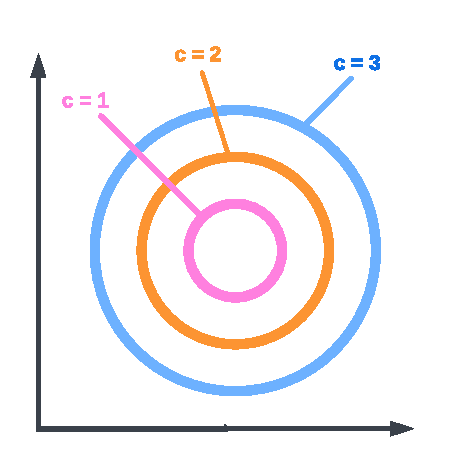
\includegraphics[scale=0.9]{./img/theory/LevelSurfaceSet.pdf}
    \caption{2D example for level surfaces for three different values.}
    \label{fig:level_surface_set}
\end{figure}

Figure \ref{fig:level_surface_set} shows level surfaces for different values of c for a 2-dimensional case. The points on the perimeter of each curve illustrate the set of points sharing the same value, i.e. $f(x_1, x_2) = c$.
\\\\
Recall that a gradient vector is defined as $\nabla f = \left[ \frac{\partial f}{\partial x_1}, \frac{\partial f}{\partial x_2}, ..., \frac{\partial f}{\partial x_d} \right]$.
\\\\
Consider a specific point $\mathbf{x}_0 \in \mathbb{R}^d$. Let us denote the level surface passing through this point by $L_{f(\mathbf{x_0})}$. Let us denote the gradient vector at $\mathbf{x_0}$ by $\nabla f_0$. 
\\\\
Now, consider an arbitrary curve $\mathbf{r}(t) = \left[x_1(t); x_2(t); \ldots, x_d(t)\right]$ (parameterized by a scalar $t$) that passes through $\mathbf{x}_0$, i.e. $\mathbf{r}(t_0) = \mathbf{x_0}$ for some $t_0 \in \mathbb{R}$. Furthermore, 
the curve $\mathbf{r}(t)$ lies within the level surface passing through $\mathbf{x}_0$, i.e. $\mathbf{r}(t) \in L_{f(\mathbf{x_0})}, \,\, \forall t$.  
\\\\
Recall that the tangent to a curve is defined as $\frac{\partial \mathbf{r}}{\partial t}$. 
\\\\
With all that context and notation behind us, now comes the `fun' part. Show that $\nabla f_0$ is orthogonal to the tangent of $\mathbf{r}(t)$ at $t_0$. 
\\\\
Now, please describe in non-technical language what you have just proven. Why might we care about this in the context of deep learning?


\taskbreak

\subsection{Bonus: Relation Gradient - Local Minimum [5 points]}
Consider a (not necessarily convex) differentiable function $g : \mathbb{R}^{n} \rightarrow \mathbb{R}$. $g$ has a local minimum at some $\mathbf{w}^{t}$ if there exists some $\gamma > 0$ such that for all $\mathbf{w} \in \mathbb{R}^{n}$, $\lVert\mathbf{w}^{t} - \mathbf{w}\rVert_{2} < \gamma \Rightarrow g(\mathbf{w}^{t}) \leq g(\mathbf{w})$.

Prove that if $g$ has a local minimum at some $\mathbf{w}^{t}$ then the gradient at $\mathbf{w}^{t} = 0$, and that the converse
is not necessarily true.


\taskbreak

\subsection{Bonus: Relation Gradient - Global Minimum [5 points]}
Prove that if a differentiable function $g : \mathbb{R}^{n} \rightarrow \mathbb{R}$ is convex and the gradient
at some $\mathbf{w}^*$ is 0, then $\mathbf{w}^*$ is the global minimum of $g$.

    
\taskbreak

\subsection{Gradient of the Softmax Function [5 points]}
We will now consider the softmax function $\mathbf{s}(\mathbf{z})$, which takes a vector input $\mathbf{z}$ and outputs a vector whose $i$-th entry $s_i$ is

\begin{equation}
    s_i = \frac{e^{z_{i}}}{\sum_{k} e^{z_{k}}}
\end{equation}

The input vector $\mathbf{z}$ to $\mathbf{s}(\cdot)$ is sometimes called the ``logits'', which just means the unscaled output of previous layers. Derive the gradient of $\mathbf{s}$ with respect to the logits, i.e. derive $\frac{\partial \mathbf{s}}{\partial \mathbf{z}}$. 



\newpage

%----------------------------------------------------------------------------------------
% Directed Acyclic Graph
%----------------------------------------------------------------------------------------
%%%%%%%%%%%%%%%%%%%%%%%%%%%%%%%%%%%%%%%%%
% Otto-Friedrich-University of Bamberg
% Chair of Explainable Machine Learning (xAI)
% Deep Learning Assignments
% LaTeX Template
% Version 1.0
%
% Author:
% Sebastian Dörrich
%%%%%%%%%%%%%%%%%%%%%%%%%%%%%%%%%%%%%%%%%

\renewcommand\thesection{\arabic{section}}
\renewcommand\thesubsection{\thesection.\arabic{subsection}}

%----------------------------------------------------------------------------------------
% Directed Acyclic Graph
%----------------------------------------------------------------------------------------
\section{Directed Acyclic Graph [10 points]}
One important property for a feed-forward network, as discussed in the lectures, is that it must be a directed acyclic graph (DAG). A \textit{DAG is a directed graph that contains no directed cycles}. We will study some of its properties in this question.
\\\\
Let's define a graph $G=(V, E)$ in which $V$ is the set of all nodes as $\{v_1, v_2, ..., v_i, ... v_n\}$ and $E$ is the set of 
edges $E = \big\{e_{i,j} = (v_i, v_j) \mid v_i, v_j \in V \big\}$.
\\\\
A \textit{topological order of a directed graph} $G=(V, E)$ is an ordering of its nodes as $\{v_1, v_2, ..., v_i, ... v_n\}$ so that for every edge $(v_i, v_j)$ we have $i < j$.
\\\\
There are several lemmas that can be inferred from the definition of a DAG. One lemma is: if $G$ is a DAG, then $G$ has a node with no incoming edges.

\medskip

\subsection{G is a DAG then G has a Topological Ordering [2 points]}
Prove that if the graph $G$ is a DAG, then $G$ has a topological ordering.


\taskbreak

\subsection{G has a Topological Ordering then G is a DAG [2 points]}
Prove that if the graph $G$ has a topological order, then $G$ is a DAG.

\taskbreak

\subsection{Computational Graphs and Backpropagation [6 points]}
For the given expression:
\begin{equation}
    A = 2\cdot \left((a + b) \cdot (a - b)\right)
\end{equation}

\vspace{0.5cm}

We can introduce intermediate variables such that there is a single mathematical operation per assignment such as:
\begin{align}
    t_1 &= a + b & t_2 &= a - b & t_3 &= t_1 \cdot t_2 & A &= 2 \cdot t_3
\end{align}

\vspace{0.5cm}

We can then use that to draw the corresponding computation graph based on the introduced variables as shown in Figure \ref{fig:computation_graph}:
\begin{figure}[h!]
    \centering
    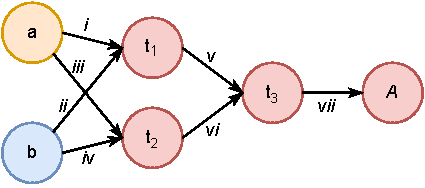
\includegraphics[scale=1.5]{./img/theory/ComputationGraph.pdf}
    \caption{Computation Graph based on the introduced intermediate variables.}
    \label{fig:computation_graph}
\end{figure}

\vspace{0.5cm}

Having the computation graph, we can write down the products of partial derivatives that are computed by a node during backpropagation for all of our nodes. Indicating to which node the results are sent to we can write:
\begin{equation}
    \begin{aligned}
        vii &\coloneqq \frac{\partial A}{\partial A} \frac{\partial A}{\partial t_3} & vi &\coloneqq \frac{\partial A}{\partial t_3} \frac{\partial t_3}{\partial t_2} & v &\coloneqq \frac{\partial A}{\partial t_3} \frac{\partial t_3}{\partial t_1} \\
        iv &\coloneqq \frac{\partial A}{\partial t_2} \frac{\partial t_2}{\partial b} &  iii &\coloneqq \frac{\partial A}{\partial t_2} \frac{\partial t_2}{\partial a} &  ii &\coloneqq \frac{\partial A}{\partial t_1} \frac{\partial t_1}{\partial b} \\
        i &\coloneqq \frac{\partial A}{\partial t_1} \frac{\partial t_1}{\partial a}
    \end{aligned}
\end{equation}

\vspace{0.5cm}

With this we can now write down the sum of partial derivative products that calculates the derivative of
the output node w.r.t. to this node for all of our nodes as:
\begin{equation}
    \begin{aligned}
        A&: \frac{\partial A}{\partial A} & t_3&: \frac{\partial A}{\partial t_3} & t_2&: \frac{\partial A}{\partial t_2} & t_1&: \frac{\partial A}{\partial t_1} \\\\
        \phantom{a}&\phantom{\frac{\partial A}{\partial t_2} \frac{\partial t_2}{\partial a} + \frac{\partial A}{\partial t_1} \frac{\partial t_1}{\partial a}} & b&: \frac{\partial A}{\partial t_2} \frac{\partial t_2}{\partial b} + \frac{\partial A}{\partial t_1} \frac{\partial t_1}{\partial b} & a&: \frac{\partial A}{\partial t_2} \frac{\partial t_2}{\partial a} + \frac{\partial A}{\partial t_1} \frac{\partial t_1}{\partial a}
    \end{aligned}
\end{equation}

\newpage

Now it is your turn. Given is the expressions:
\begin{equation}
    \begin{aligned}
        A &= \frac{{\rm e}^{a}}{\sqrt{b}} \log \left(a + b\right) \\
        % B &= \sqrt{a + b + c^2} + \log\left(a + b + c^2 \right) + \frac{a + b + c^2}{bc^2} \\
        % C &= \sum_{i=1}^{3} \left(w_0 + w_1 x_i - y_i \right)^2
    \end{aligned}
\end{equation}
\begin{itemize}
    \item[a)] Introduce intermediate variables ($t_1$, $t_2$, $t_3$, ...) such that there is a single mathematical operation per assignment. Reuse intermediate variables whenever possible.
    \subtaskbreak

    \item[b)] Draw the corresponding computation graph based on the variables you introduced in a).
    \subtaskbreak
    
    \item[c)] For each edge in your computation graph, write down the products of partial derivatives $\left(\text{e.g. } \frac{\partial \mathcal{L}}{\partial y} \frac{\partial y}{\partial x}\right)$ that are computed by this edge during backpropagation. For each such product indicate to which node the results are sent to (e.g. by writing down the products close to the corresponding graph edges).\\
    Note: you do not need to symbolically calculate or simplify the derivative for specific operations.
    \subtaskbreak
    
    \item[d)] At each node, write down the sum of partial derivative products that calculates the derivative of the output node w.r.t. to this node. Your expressions only need to contain the direct children for the node and again you do not need to symbolically calculate or simplify the derivatives.
\end{itemize}



\newpage

%----------------------------------------------------------------------------------------
% Logistic Regression
%----------------------------------------------------------------------------------------
%%%%%%%%%%%%%%%%%%%%%%%%%%%%%%%%%%%%%%%%%
% Otto-Friedrich-University of Bamberg
% Chair of Explainable Machine Learning (xAI)
% Deep Learning Assignments
% LaTeX Template
% Version 1.0
%
% Author:
% Sebastian Dörrich
%%%%%%%%%%%%%%%%%%%%%%%%%%%%%%%%%%%%%%%%%

\renewcommand\thesection{\arabic{section}}
\renewcommand\thesubsection{\thesection.\arabic{subsection}}

%----------------------------------------------------------------------------------------
% Logistic Regression
%----------------------------------------------------------------------------------------
\section{Logistic Regression [5 points]}
Using the chain rule, show that:
\begin{equation}
    \nabla_{\mathbf{w}} \frac{1}{B} \sum_{i=1}^{B} \mathcal{L} \left(y_i, \hat{y}_i \right) = \frac{1}{B} \sum_{i=1}^{B} \left(\hat{y}_i - y_i \right) \mathbf{x}_i
\end{equation}
where
\begin{equation}
    \begin{aligned}
        \mathcal{L} \left(y_i, \hat{y}_i \right) &= -y \log \left(\hat{y}\right) - \left(1 - y\right) \log \left(1 - \hat{y} \right) \\
        \hat{y}_i &= \sigma\left(\mathbf{w}^\intercal \mathbf{x}_i \right)
    \end{aligned}
\end{equation}



\end{document}